%%%%%%%%%%%%%%%%%%%%%%%%%%%%%%%%%%%%%%%%%%%%%%%%%%%%%%%%%%%%%%%%%%%%%%%%%%%%%%%%%%%%%%
%  File 52_online_nesting.tex
%%%%%%%%%%%%%%%%%%%%%%%%%%%%%%%%%%%%%%%%%%%%%%%%%%%%%%%%%%%%%%%%%%%%%%%%%%%%%%%%%%%%%%

\section{ドメインネスティング実験} \label{sec:nest_exp}
%====================================================================================

本節では、SCALEでネスティング実験を行う方法について説明する。ネスティング実験とは、図\ref{fig_nestsample}に
示すように、水平格子間隔の異なる複数の計算領域(ドメイン)を設定し、領域が重複するように入れ子(ネスト)構造に
することで、広領域かつ高解像度のドメインを設定する計算領域設定方法である。図\ref{fig_nestsample}の例では、
3つのドメインを用いた3段ネスティング構成になっている。外側のドメインは比較的粗い
水平解像度であるが広い領域を取ることで大きな場の構造を表現することができる。逆に内側のドメインは、比較的狭い
領域であるが細かい水平解像度を取ることで対象とする現象の細かい構造を表現することができる。ここでは、
入れ子構造のうち、データを渡す側のドメインを「親ドメイン」、データを受ける側のドメインを「子ドメイン」と称する。

SCALEはオフライン・ネスティング実験とオンライン・ネスティング実験の両方をサポートしている。オフライン・ネスティング実験は、
はじめに親ドメインだけで時間積分を行い、その計算結果のhistoryデータを用いて、子ドメイン用の初期値・境界値を作成する。
その後に子ドメインの時間積分を行う。オンライン・ネスティング実験は、親ドメインと子ドメインを同時に実行し、適宜計算途中の
データを親ドメインから子ドメインへMPI通信によって受け渡しすることで、子ドメインの時間積分を行う。
オンライン・ネスティング実験が実行できる計算機リソースがあれば、オンラインで実行することを推奨する。
それは、オンラインの場合、子ドメインの境界条件の更新間隔は親ドメインの時間積分間隔に一致するため、
可能な限り細かい境界条件の更新間隔を得ることができる。また、中間ファイルも作成されずディスクリソースにも優しい。

ドメインネスティング実験を行う上で共通する実験設定の制限事項は、基本的に以下の2点だけである。
\textcolor{red}{
\begin{itemize}
 \item 親ドメインの領域は子ドメインの領域を完全に内包しなければならない。
 \item 親ドメインの積分時間は子ドメインの積分時間を完全に内包しなければならない。
\end{itemize}
}

これに加えて、オンライン・ネスティング実験の場合、現在のところ親ドメインと子ドメインの積分時間は一致させなければならない。
SCALEではオンライン・ネスティングであっても、親ドメインと子ドメインの間で鉛直層数、鉛直層設定、地図投影法、そして
物理スキームが異なっていても構わない。

オフライン、オンラインに関わらず、ドメイン間の格子間隔比率($DX_{parent}/DX_{child}$)にシステム上は制限はないが、
この比率が大きすぎると計算結果の物理的なパフォーマンスが下がる可能性がある。本書では5倍以下で使用することを推奨する。

以降、まずは実行方法がわかりやすいオフライン・ネスティング実験から説明し、ついでオンライン・ネスティング実験に
ついて説明する。configファイルの名前に特に指定はないが、ここでの表記としては、
\textcolor{blue}{``***.parent.conf''と表記すれば、親ドメインのconfigファイルを編集する}ことを意味し、
\textcolor{blue}{``***.child.conf''と表記すれば、子ドメインのconfigファイルを編集する}ことを意味する。


\begin{figure}[t]
\begin{center}
  
\includegraphics[width=1.0\hsize]{./figure/nesting_sample.eps}\\
  \caption{日本の近畿地方を対象領域としたドメインネスティング設定の例. domain 1が最外ドメインでdomain 3が最内ドメインである。
           赤い矩形と線は、それぞれの位置関係を示している。domain 1の水平格子間隔は7.5 km、domain 2は2.5 km、
           そしてdomain 3は0.5 kmである。}
  \label{fig_nestsample}
\end{center}
\end{figure}


\subsection{オフライン・ネスティング実験の方法} \label{sec:nest_offline}
%------------------------------------------------------

ここでは、親ドメインは解像度は荒いが広領域の外側ドメインで、子ドメインは領域は狭いが高解像度の内側ドメインで
あることを想定する。このとき、2段ネスティングのオフライン・ネスティング実験の実行過程は次のようになる。

{\gt
\begin{enumerate}
 \item 親ドメインの時間積分計算を行う。
 \item 親ドメインの出力ファイル(history)を用いて子ドメインの初期値/境界値を作成する。
 \item 作成した初期値/境界値を用いて子ドメインの時間積分計算を行う。
\end{enumerate}
}

以下、この流れに沿って説明を進める。親ドメインと子ドメインそれぞれについて、``pp.***.conf''、``init.***.conf''、
そして``run.***.conf''ファイルを事前に作成し、親ドメイン、子ドメインともに地形/土地利用データの作成を終え、
親ドメインについては、初期値/境界値データの作成を終えていることを想定して説明を進める。
ここで説明するオフライン・ネスティング実験の設定を記述したconfigファイルがチュートリアルディレクトリの下、
``tutorial/real/sample/offline\_nesting''に置いてあるので、説明を読み進める上で参考にしてもらいたい。

\subsubsection{親ドメインの時間積分計算を行う}
基本的には通常のシングルドメインの計算と同じ方法で実行すればよいが、``run.conf''ファイルの設定について、
次の3点の注意点・変更点がある。

\begin{itemize}
 \item 親ドメインのhistory出力間隔を適度に細かくとること。
 \item 親ドメインのhistory出力形式で\verb|ZINTERP|は``false''に設定すること。
 \item 親ドメインのhistory出力形式で\verb|STEP0|は``true''に設定すること。
 \item 親ドメインの計算領域を子ドメインへ伝える「カタログファイル」を出力すること。
\end{itemize}


この設定を``run.parent.conf''に適用すると下記のようになる。赤文字で示した部分が、
上記の注意点・変更点に対応する部分である。\\

\noindent {\small {\gt
\ovalbox{
\begin{tabularx}{140mm}{l}
\textcolor{red}{\verb|&PARAM_DOMAIN_CATALOGUE|} \\
\textcolor{red}{\verb| DOMAIN_CATALOGUE_OUTPUT = .true.,|} \\
\textcolor{red}{\verb|/|} \\
 \\
\verb|&PARAM_HISTORY| \\
\verb| HISTORY_DEFAULT_BASENAME  = "history",| \\
\textcolor{red}{\verb| HISTORY_DEFAULT_TINTERVAL = 600.D0,|} \\
\verb| HISTORY_DEFAULT_TUNIT     = "SEC",| \\
\verb| HISTORY_DEFAULT_TAVERAGE  = .false.,| \\
\verb| HISTORY_DEFAULT_DATATYPE  = "REAL4",| \\
\textcolor{red}{\verb| HISTORY_DEFAULT_ZINTERP   = .false.,|} \\
\textcolor{red}{\verb| HISTORY_OUTPUT_STEP0      = .true.,|} \\
\verb|/| \\
\end{tabularx}
}}}\\

\verb|PARAM_DOMAIN_CATALOGUE|の項目の``\verb|DOMAIN_CATALOGUE_OUTPUT|''の変数がカタログファイルの出力設定である。
もともとのconfigファイルには項目自体がないこともあるので、その場合は自分で項目を加えて設定すること。
カタログファイルは、``latlon\_domain\_catalogue.txt''というファイル名で出力される。この中には、MPIプロセス毎に分割
して担当した計算領域の四隅の緯度・経度が記述されている。

\verb|HISTORY_DEFAULT_TINTERVAL|の設定項目によってhistoryデータ出力間隔を指定する(単位は秒である)。指定値に
任意性はあるが、子ドメインの側面境界条件の更新間隔として使用可能であると考えられる範囲で指定すること。
親ドメイン、子ドメインの解像度、および実行環境のディスク空き容量にもよるが、おおよそ最大で1時間間隔、
出来れば10分間隔のhistoryデータ出力間隔を指定することが多い。

設定が完了すれば、``scale-les''を実行して親ドメインの時間積分計算を行う。


\subsubsection{親ドメインの出力ファイルを用いて子ドメインの初期値/境界値を作成する}
次に計算が終わった親ドメインのhistoryデータ出力を用いて、子ドメインの初期値/境界値を作成する。
実行するプログラムは、通常の初期値/境界値作成と同じ``scale-les\_init''だが、
``init.child.conf''を下記のように編集する。\\

\noindent {\small {\gt
\ovalbox{
\begin{tabularx}{140mm}{l}
\verb|&PARAM_MKINIT_REAL| \\
\verb| BASENAME_BOUNDARY   = "boundary",| \\
\textcolor{red}{\verb| BASENAME_ORG        = "history",|} \\
\textcolor{red}{\verb| FILETYPE_ORG        = "SCALE-LES",|} \\
\textcolor{red}{\verb| NUMBER_OF_TSTEPS    = 25,|} \\
\textcolor{red}{\verb| BOUNDARY_UPDATE_DT  = 600.D0,|} \\
\verb|/| \\
 \\
\textcolor{red}{\verb|&PARAM_NEST|} \\
\textcolor{red}{\verb| USE_NESTING               = .true.,|} \\
\textcolor{red}{\verb| OFFLINE                   = .true.,|} \\
\textcolor{red}{\verb| OFFLINE_PARENT_PRC_NUM_X  = 4,|} \\
\textcolor{red}{\verb| OFFLINE_PARENT_PRC_NUM_Y  = 4,|} \\
\textcolor{red}{\verb| OFFLINE_PARENT_KMAX       = 35,|} \\
\textcolor{red}{\verb| OFFLINE_PARENT_IMAX       = 40,|} \\
\textcolor{red}{\verb| OFFLINE_PARENT_JMAX       = 40,|} \\
\textcolor{red}{\verb| OFFLINE_PARENT_LKMAX      = 5,|} \\
\textcolor{red}{\verb| LATLON_CATALOGUE_FNAME    = "latlon_domain_catalogue.txt",|} \\
\textcolor{red}{\verb|/|} \\
\end{tabularx}
}}}\\

\noindent 読み込む外部入力データのファイル名を指定する``\verb|BASENAME_ORG|''は、親モデルのhistory.pe***.nc
ファイルを読み込むので、``history''と指定する。また、このhistoryファイルはSCALE-LESモデルの出力データなので、
``\verb|FILETYPE_ORG|''は、``SCALE-LES''と指定する。\verb|NUMBER_OF_TSTEPS|には、historyファイルが持つ時間ステップ数
を記述する(例として25が記述されているだけ)。\verb|BOUNDARY_UPDATE_DT|には、時間ステップの時間間隔を指定する
(単位は秒である)。つまり、親ドメインの\verb|HISTORY_DEFAULT_TINTERVAL|の設定項目に一致する値を指定する。
この説明では、親ドメインで600秒としたので、ここでも600秒を指定する。

\verb|PARAM_NEST|の項目は、ネスティング実験のために新たに加える項目である。もともとのconfigファイルには項目自体がないので、
自分でconfigファイルに追記する。最初の2つの項目によって、オフライン・ネスティング実験であることが決定される。
``\verb|OFFLINE_PARENT_|''で始まる6つの設定変数は、親ドメインの設定を記述する変数である。親ドメインの対応する項目を
参照して正しく設定すること。この例では、親ドメインは$4 \times 4$のMPIプロセス数を使用し、鉛直35層で、水平には1つの
MPIプロセスあたり$40 \times 40$の格子点を持っており、陸面モデルは5層モデルであることを想定している。
最後の``\verb|ATLON_CATALOGUE_FNAME|''の項目は、親ドメインを実行した時に出力したカタログファイルを指定する。

設定の編集が完了すれば、``scale-les\_init''を実行して子ドメインの初期値/境界値を作成する。\\

\noindent {\small {\gt
\fbox{
\begin{tabularx}{140mm}{l}
\verb|xxx ERROR: REQUESTED DOMAIN IS TOO MUCH BROAD| \\
\verb|xxx -- LONGITUDINAL direction over the limit| \\
\end{tabularx}
}}}\\

\noindent 実行時に上記のようなメッセージが表示されて計算が止まる場合は、子ドメインの計算領域が親ドメインの計算領域の
外側に取られている部分がある。この場合は、各ドメインの大きさや領域中心の設定を見直す必要がある。


\subsubsection{作成した初期値/境界値を用いて子ドメインの時間積分計算を行う}
初期値/境界値作成が終われば、子ドメインの時間積分計算を実行する。子ドメインの実行は、通常の現実大気実験と何も変わらないので、
必要なデータのPATHが正しくconfigファイルに記述されていることを確認してから、``scale-les''を実行すればよい。

1点だけ設定を忘れやすい設定項目を挙げておく。\\

\noindent {\small {\gt
\ovalbox{
\begin{tabularx}{140mm}{l}
\verb|&PARAM_MKINIT_REAL| \\
\verb|     〜 中略 〜|\\
\textcolor{red}{\verb| BOUNDARY_UPDATE_DT  = 600.D0,|} \\
\verb|/| \\
\end{tabularx}
}}}\\

\noindent ``run.child.conf''の\verb|BOUNDARY_UPDATE_DT|を、初期値/境界値作成で使用した親ドメインの
historyデータ出力間隔に合わせておくことを忘れないようにすること。オフライン・ネスティング実験の場合、
現在のところこの設定に親ドメインと子ドメイン間で不整合あっても警告やエラーメッセージが発せられないまま、
時間積分計算が進み、場合によっては正常終了してしまうため注意が必要である。

多段のオフライン・ネスティング実験を行いたい場合は、ここまでの過程を繰り返せばよい。つまり、子ドメインとして
時間積分計算した結果を再度、親ドメインと見立てて、さらに内側の孫ドメインの初期値/境界値作成を行なえばよい。
以上でオフライン・ネスティングの実行方法の説明を終える。


\subsection{オンライン・ネスティング実験の方法} \label{sec:nest_online}
%------------------------------------------------------

オフライン・ネスティング実験では、各ドメインの計算を逐次的に実行する必要があったが、オンライン・ネスティング実験では
全てのドメインの計算を同時に実行する。現在は、親ドメインから子ドメインへのみデータ受け渡しを行う、いわゆる
``1-Wayネスティング''のみをサポートしている。オンライン・ネスティング実験でサポートするネスティング段数は、
最大で10段までである。

SCALEのオンライン・ネスティング実験は、複数のドメインを逐次的に時間積分計算を進めるのではなく、並列的に時間積分計算を行う。
図\ref{fig_mpisplit}に示すイメージ図のように、与えられたMPIプロセスを分割してそれぞれのドメインに分配し、各々のドメインが
独立したモデルのように計算を進める。後ほど説明するが、複数のドメインを立ち上げるために実行時には``launch.conf''という
起動用のconfigファイルが別途必要になる。

\begin{figure}[t]
\begin{center}
  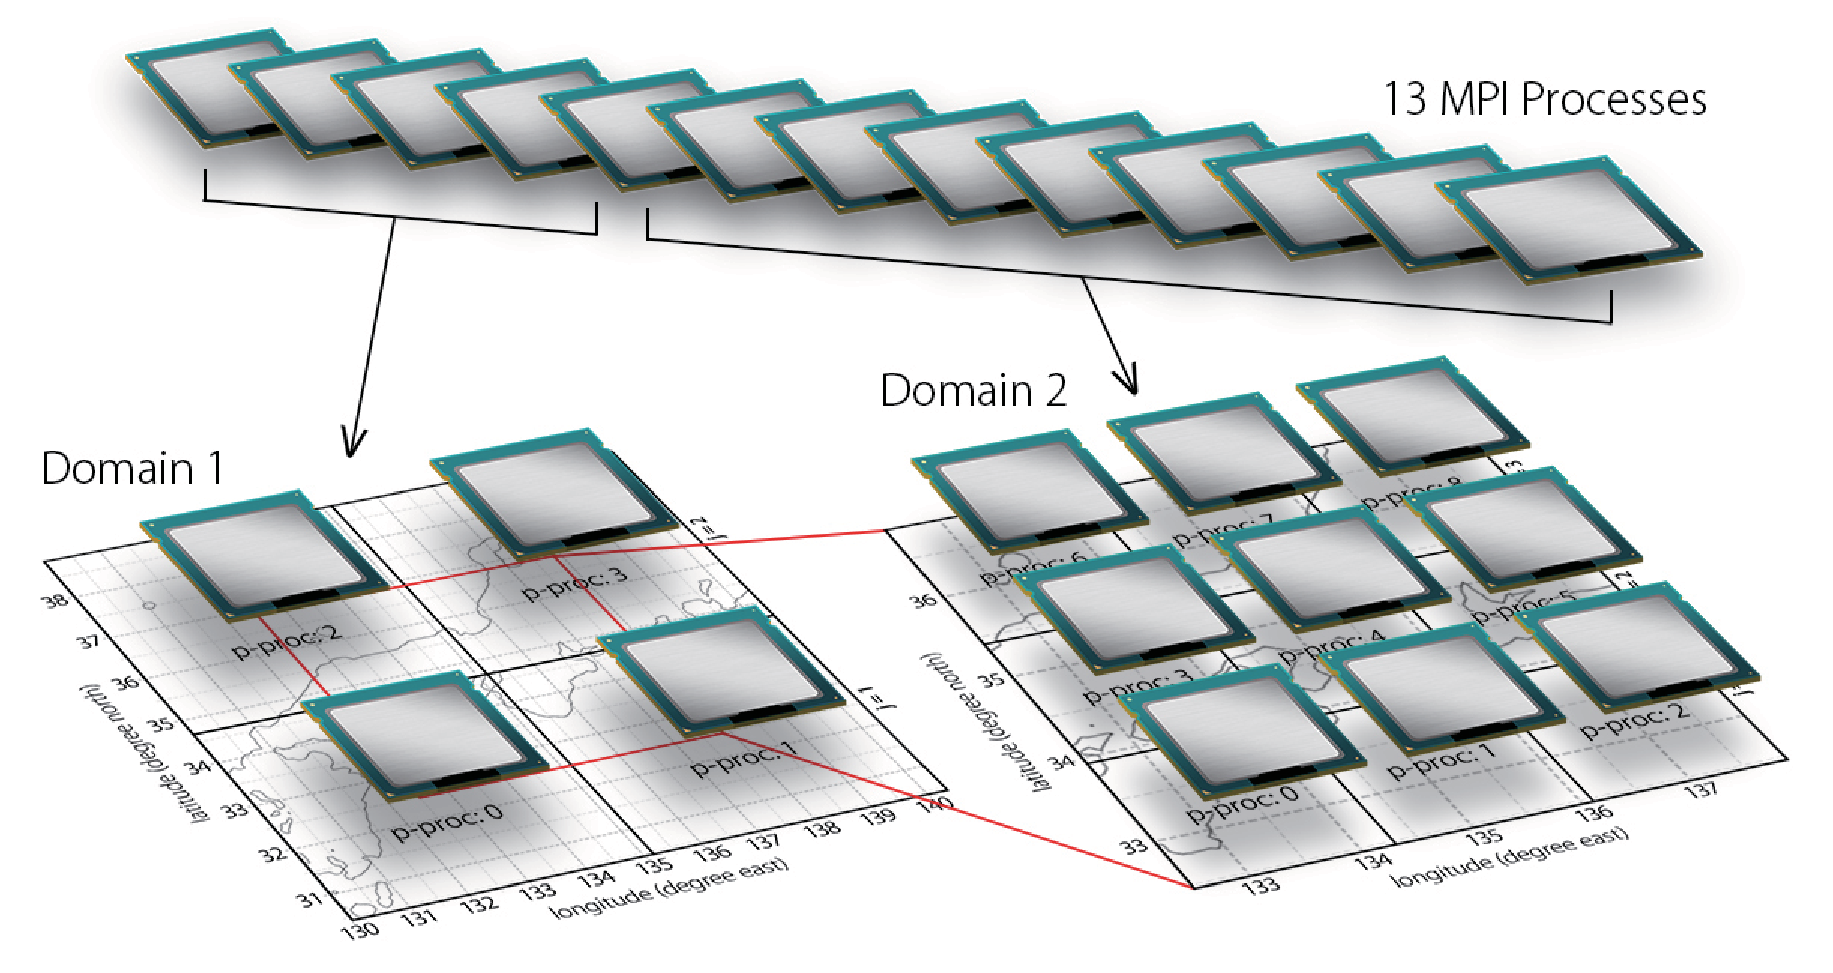
\includegraphics[width=0.8\hsize]{./figure/mpisplit_nesting.eps}\\
  \caption{オンライン・ネスティング実験のMPIプロセス配分イメージ. 全部で13のプロセスを立ち上げ、これを適切に分配することで、
           Domain 1は$2 \times 2$の4-MPI並列、Domain 2は$3 \times 3$の9-MPI並列計算を行う。Domain 1からDomain 2へMPI通信
           によってデータを受け渡ししながら時間積分計算を進める。}
  \label{fig_mpisplit}
\end{center}
\end{figure}


ここでは、最も単純な2段ネスティングの例を説明する。親ドメインは解像度は荒いが広領域の外側ドメインで、
子ドメインは領域は狭いが高解像度の内側ドメインであることを想定する。

オンライン・ネスティング実験を行う場合は、``scale-les''のモデル本体実行前に全てのドメインについて、
地形/土地利用データの作成、及び初期値/境界値データの作成を事前に行っておく必要がある。従って、親ドメインと子ドメイン
それぞれについて、``pp.***.conf''、``init.***.conf''、そして``run.***.conf''ファイルを事前に作成し、
親ドメイン、子ドメインともに地形/土地利用データの作成、及び初期値/境界値データの作成を終えていることを想定して説明を進める。
ここで説明するオンライン・ネスティング実験の設定を記述したconfigファイルがチュートリアルディレクトリの下、
``tutorial/real/sample/online\_nesting''に置いてあるので、説明を読み進める上で参考にしてもらいたい。


\subsubsection{configファイルの編集}
まず、親ドメイン、子ドメインそれぞれに``run.***.conf''ファイルを編集する。

\noindent {\gt \verb|run.parent.conf|の編集内容}\\
{\small {\gt
\ovalbox{
\begin{tabularx}{140mm}{l}
\verb|&PARAM_NEST| \\
\verb| USE_NESTING              = .true.,| \\
\verb| OFFLINE                  = .false.,| \\
\verb| ONLINE_DOMAIN_NUM        = 1,| \\
\verb| ONLINE_IAM_PARENT        = .true.,| \\
\verb| ONLINE_IAM_DAUGHTER      = .false.,| \\
\verb| ONLINE_BOUNDARY_USE_QHYD = .true.,| \\
\verb| ONLINE_AGGRESSIVE_COMM   = .true.,| \\
\verb|/| \\
\end{tabularx}
}}}\\

\vspace{0.5cm}

\noindent {\gt \verb|run.child.conf|の編集内容}\\
{\small {\gt
\ovalbox{
\begin{tabularx}{140mm}{l}
\verb|&PARAM_NEST| \\
\verb| USE_NESTING              = .true.,| \\
\verb| OFFLINE                  = .false.,| \\
\verb| ONLINE_DOMAIN_NUM        = 2,| \\
\verb| ONLINE_IAM_PARENT        = .false.,| \\
\verb| ONLINE_IAM_DAUGHTER      = .true.,| \\
\verb| ONLINE_BOUNDARY_USE_QHYD = .true.,| \\
\verb| ONLINE_AGGRESSIVE_COMM   = .true.,| \\
\verb|/| \\
\end{tabularx}
}}}\\

\noindent 上記の\verb|PARAM_NEST|の項目は、ネスティング実験のために新たに加える項目である。
もともとのconfigファイルには項目自体がないので、自分でconfigファイルに追記する。最初の2つの項目によって、
オンライン・ネスティング実験であることが決定される。``\verb| ONLINE_|''で始まる設定変数はオンライン・ネスティング実験
専用の設定変数である。\verb|ONLINE_DOMAIN_NUM|は、ドメインのID番号であり、外側ドメインから内側ドメインへ順番に
番号を振っていく。ここでは、親ドメインは1番、子ドメインは2番と設定する。

\verb|ONLINE_IAM_PARENT|と\verb|ONLINE_IAM_CHILD|は各ドメインの役割を設定するパラメータである。
これらの変数は、``In online nesting system, I am parent (or, I am child).''という意味で覚えれば設定を間違うことはない。
少し脇道にそれるが、ここで説明している設定より複雑なものとして、図\ref{fig_nestsample}のような
3段ネスティング実験の場合の設定例を表\ref{tab:triple_nested}に示した。

\begin{table}[htb]
\begin{center}
\caption{3段ネスティング実験の設定例}
\begin{tabularx}{150mm}{|l|l|l|X|} \hline
 \rowcolor[gray]{0.9} ドメイン & \verb|ONLINE_DOMAIN_NUM| & \verb|ONLINE_IAM_PARENT| & \verb|ONLINE_IAM_CHILD|\\ \hline
 最外ドメイン & 1 & \textcolor{blue}{true} & \textcolor{red}{false} \\ \hline
 中間ドメイン & 2 & \textcolor{blue}{true} & \textcolor{blue}{true} \\ \hline
 最内ドメイン & 3 & \textcolor{red}{false} & \textcolor{blue}{true} \\ \hline
\end{tabularx}
\label{tab:triple_nested}
\end{center}
\end{table}

\noindent 最外ドメインは親ドメインとしてのみ働き、最内ドメインは子ドメインとしてのみ働く。一方、中間ドメインは最外ドメインに
対しては子ドメイン、最内ドメインに対しては親ドメインとして働くため両方共``true''となる。

さて、configファイルの編集内容の説明に戻る。\verb|ONLINE_BOUNDARY_USE_QHYD|は、「側面境界条件として親ドメインの凝結物の
混合比を使うかどうか」を指定する設定変数である。外部入力データから側面境界条件を作成するときには通常使わないが、
ネスティングの場合、ドメイン間の物理スキームの違いがなかったり、解像度もそれほど大きく離れていないため、側面境界から
凝結物自体が移流して入ってくる設定も選択肢に入るだろう。側面境界付近で雲が立ちにくい問題を解決したり、親ドメインとの乖離を
抑制したりする可能性がある。

最後の\verb|ONLINE_AGGRESSIVE_COMM|はオンライン・ネスティング時のドメイン間通信に関する最適化変数である。
通常は、``true''と設定して実行する。


\subsubsection{launchファイルの編集}
オンライン・ネスティング実験の実行には、``run.***.conf''の他に、起動用configファイル``launch.conf''が必要である。
\begin{verbatim}
 $ vi launch.conf
\end{verbatim}
などとして、適宜エディタをたちあげて新規ファイルを作成し、下記の内容を記述する。\\

\noindent {\small {\gt
\ovalbox{
\begin{tabularx}{140mm}{l}
\verb|&PARAM_LAUNCHER| \\
\verb| NUM_DOMAIN  = 2,| \\
\verb| CONF_FILES  = run.parent.conf,run.child.conf,| \\
\verb| PRC_DOMAINS = 4,9,| \\
\verb|/| \\
\end{tabularx}
}}}\\

\noindent 図\ref{fig_mpisplit}のイメージを思い浮かべながら設定を確認してもらいたい。\verb|PARAM_LAUNCHER|の項目のうち、
\verb|NUM_DOMAIN = 2|が「2つのドメインを起動する」ことを表しており、\verb|CONF_FILES|の項目に羅列されたファイル名は、
各々のドメインで読み込むconfigファイルを指定している。\verb|PRC_DOMAINS|は各々のドメインで使用するMPIプロセス数を
指定する。\verb|PRC_DOMAINS|は、\verb|CONF_FILES|で羅列した順番で指定しなければならない。従ってこの場合、
親ドメインは4-MPI並列、子ドメインは9-MPI並列で実行するように指定されている。ここで指定するMPIプロセス数は、
各々の``run.***.conf''で指定されている総MPIプロセス数と合致させなければならない。
この2段オンライン・ネスティング実験で使用する総MPIプロセス数は、$4 + 9 = 13$プロセスとなる。

実行時には、シングルドメイン計算とは異なり、\verb|launch.conf|を引数に指定し、計算全体で使用するMPIプロセス数を
指定して実行する。
\begin{verbatim}
 $ mpirun  -n  13  ./scale-les  launch.conf
\end{verbatim}

実行にあたって注意することは、複数のドメインの計算を同時に実行するため、\textcolor{red}{ドメイン間でconfigファイルに
記述された出力ファイル名をドメイン毎に変更しなければならない}ことである。たとえば,``history.pe***.nc''は、
``history\_d01.pe***.nc''、``history\_d02.pe***.nc''といったようにドメイン毎に名前を変えながらどのドメインの
出力データであるか判別がつくようにconfigファイルの記述を設定する。
historyファイルのほかに、LOGファイル、topoファイル、landuseファイル、boundaryファイル、initファイル、restartファイル、
そしてmonitorファイルの名前を変更しておく必要がある。

実行時に次のようなエラーメッセージが出力されて計算が異常終了することがある。\\

\noindent {\small {\gt
\fbox{
\begin{tabularx}{140mm}{l}
\verb|xxx region of daughter domain is larger than that of parent: SW search| \\
\end{tabularx}
}}}\\

\noindent {\small {\gt
\fbox{
\begin{tabularx}{140mm}{l}
\verb|xxx region of daughter domain is larger than that of parent: NE search| \\
\end{tabularx}
}}}\\

\noindent これは、子ドメインで設定された計算領域が親ドメインの計算領域よりも大きいことを意味するエラーメッセージである。
``SW search''のエラーが出る場合は子ドメインの西側か南側が親ドメインの外側に出ており、``NE search''のエラーが出る場合は
子ドメインの東側か北側が親ドメインの外側に出ていることを意味している。再度設定を確認し、地形・土地利用データ、および
初期値/境界値作成からやり直すこと。


\subsubsection{MPIプロセスの分配ガイドライン}
SCALEのオンライン・ネスティング実験は、図\ref{fig_mpisplit}のイメージ図で説明したように、MPIプロセスを分割し、複数のドメイン
に分配する。現在のところ、その分配割合はユーザーに委ねられているため、適切にMPIプロセスを分配しなければ余計な計算時間が
かかってしまう。ここでは、適切にMPIプロセスを分配するためのガイドラインについて説明する。ガイドラインは、ドメイン毎に
\textcolor{blue}{「単位あたりの時間積分にかかる1プロセスあたりの演算量を揃える」}という単純なものである。
ここでは、以下に示す2段オンライン・ネスティング実験を行う場合を想定し、ガイドラインに沿ったプロセス分配方法の例を示す。
``domain 1''は外側の親ドメイン、``domain 2''は内側の子ドメインを意味する。

\begin{table}[htb]
\begin{center}
\caption{2段オンライン・ネスティング実験の設定想定}
\begin{tabularx}{150mm}{|l|l|X|} \hline
 \rowcolor[gray]{0.9} 設定項目 & domain 1 & domain 2 \\ \hline
 計算領域 & 450 km $\times$ 450 km & 200 km $\times$ 200 km \\ \hline
 DX \& DY(X,Y同一設定) & 3 km & 1 km \\ \hline
 鉛直層設定 & 40層 & 60層 \\ \hline
 積分時間間隔(DT)& 30 sec & 10 sec \\ \hline
 積分時間 & 3600 sec & 3600 sec \\ \hline
\end{tabularx}
\label{tab:nest_proc_guide1}
\end{center}
\end{table}

このとき、親ドメインの水平方向の一辺の格子点数は、$450 km \div 3 km = 150$点であるので、総格子点数は
$X \times Y \times Z = 150 \times 150 \times 40 = 900,000$点である。一方、子ドメインの水平方向の一辺の格子点数は、
$200 km \div 1 km = 200$点であるので、総格子点数は$200 \times 200 \times 60 = 2,400,000$点である。1つの時間ステップの
積分を行うのにこれだけの格子点について計算を行わなければならない。

積分時間間隔は格子間隔に依存するためにドメイン毎に異なる。この例では、domain 1は30 secだが、domain 2は10 secであり、
3倍の差がある。したがって、同じ30 secという積分時間に対してdomain 2は3倍多くの時間ステップ、つまり3倍の演算量を要する。
これらを考慮して、簡単なドメイン間の演算量比率(Computation Rate)の指標を考えると下記の式で表される。
\begin{eqnarray}
ComputationRate=\frac{Xgrd_{child} \times Ygrd_{child} \times Zgrd_{child} \times Ustep_{child}}
                     {Xgrd_{parent} \times Ygrd_{parent} \times Zgrd_{parent} \times Ustep_{parent}} \nonumber
\end{eqnarray}
ここで、Xgrd、Ygrd、ZgrdはそれぞれX方向、Y方向、Z方向の格子点数を表し、Ustepは単位時間積分に必要な時間ステップ数を表す。
ここでの例をこの式に当てはまると、演算量比率は$(2,400,000 \times 3) \div (900,000 \times 1) = 8$であることがわかる。
おおよそ、この割合にしたがってMPIプロセスをドメイン毎に分配すればよい。例えばdomain 1は4プロセス、domain 2は32プロセスを
使用し、全体で36プロセスを使用する設定が考えられる。この場合、例えば次のように設定することができる。

\begin{table}[htb]
\begin{center}
\caption{2段オンライン・ネスティング実験のMPIプロセス設定例}
\begin{tabularx}{150mm}{|l|l|X|} \hline
 \rowcolor[gray]{0.9} 設定項目 & domain 1 & domain 2 \\ \hline
 MPIプロセス(X $\times$ Y) & 2 $\times$ 2 & 4 $\times$ 8 \\ \hline
 水平格子点数(IMAX $\times$ JMAX) & 75 $\times$ 75 & 50 $\times$ 25 \\ \hline
\end{tabularx}
\label{tab:nest_proc_guide2}
\end{center}
\end{table}

X方向とY方向に分配するプロセス数には任意性が残るが、この例のdomain 2のようにXとYで大きくプロセス数が異なる場合には、
X方向の格子点数(IMAX)の値が大きくなる設定を取ると計算機の演算性能を引き出しやすいと考えられる\footnote{SCALEでは
X方向のDo Loopが最も最内ループになっているため、X方向の回転数が多いとプリフェッチ機能が効果を発揮しやすく、メモリ性能
へのプレッシャーが緩和される。ただし、京の場合のようにスレッド並列も併用するハイブリッド並列の場合にはY方向の格子点数
もある程度大きくしてスレッド間の演算量のインバランスを小さくする必要性も出てくる。}。

この設定は一例であり、これ以外の方法で設定しても構わない。また、ここでは格子点数と積分時間間隔だけに着目して演算量比率
を考えたが、実際の計算には様々な物理過程も含まれるだろうし、それらをCallする時間間隔もドメイン毎に異なるかもしれない。
さらにドメイン内通信やドメイン間通信のMPI通信にかかる時間も影響を及ぼす。SCALEにおけるオンライン・ネスティングの実装に
おいて最も重要なことは、最内ドメインが時間積分を実行し続けることである。同じ設定で何度も実験を行うような場合には、上記の
方法である程度の見通しをつけた上で、いくらかの微調整を行うことをおすすめする。
以上でオンライン・ネスティングの実行方法の説明を終える。


\subsection{子ドメインにおける地形の取り扱い} \label{sec:nest_topo}
%------------------------------------------------------
ネスティング実験を行う際、ドメイン間の格子間隔比率が大きい場合などに子ドメインのバッファー領域内で不整合が発生する
可能性がある。バッファー領域内は親ドメインの計算結果を用いて一部の変数にダンピングがかかるが、地形の表現性が異なる
ことで、子ドメインにとっては正しくない値へダンピングされる可能性がある。例えば、子ドメインでは斜面上の小さな谷として
表現されている地形が、親ドメインでは格子間隔が荒く谷がなくスムースな斜面として表現される場合が考えられる。

こういった不整合を無くすために、バッファー領域では親ドメインの地形を用い、内側領域では子ドメイン自身の地形を用いる
「地形コピー」の機能が実装されている。この機能を使えば、図\ref{fig_topocopy}に示すようにバッファー領域は完全に
親ドメインに一致する地形で、内側に移る地形遷移領域内では親ドメインと子ドメインのミックス、それより内側では完全に
子ドメインの地形という設定を構築することができる。以降、その設定方法と実行手順を説明する。基本的には、
オフライン・ネスティングのフレームワークを利用して進める。
ここで説明する地形コピーの設定を記述した``pp.d0*.conf''ファイルがチュートリアルディレクトリの下、
``tutorial/real/sample/online\_nesting''に置いてあるので、説明を読み進める上で参考にしてもらいたい。

\begin{figure}[tb]
\begin{center}
  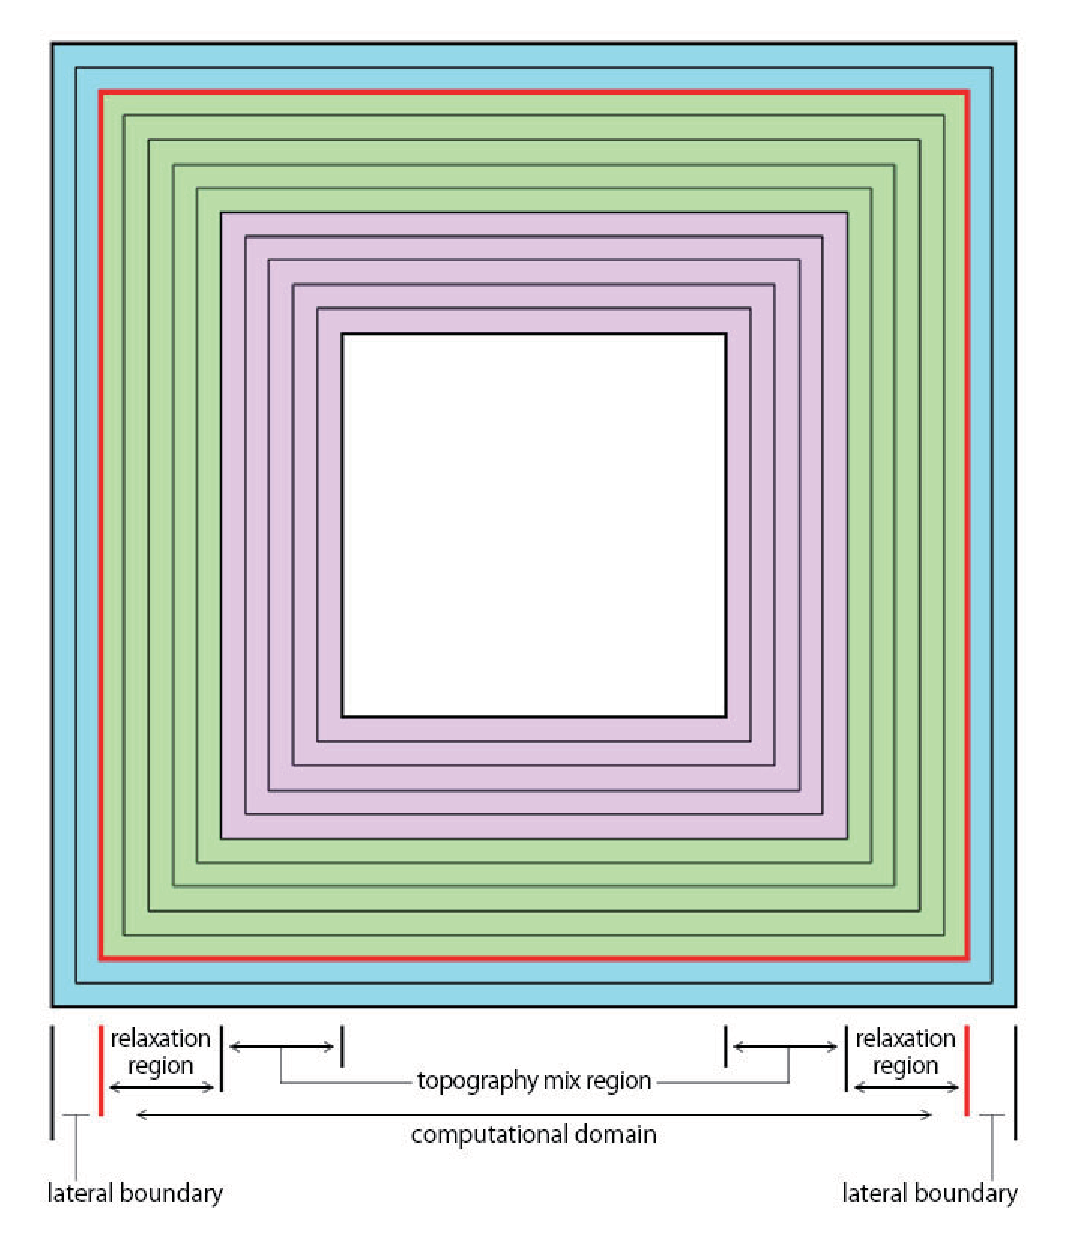
\includegraphics[width=0.4\hsize]{./figure/topo_copy.eps}\\
  \caption{地形コピーを適用した子ドメインの地形データ水平分布. 最外の水色の2層は側面境界で、それより内側の赤色の線で
           囲われた領域が計算領域である。緑色の部分がバッファー領域、桃色の部分が地形遷移領域、そして最内の白色の
           部分が子ドメインの地形をもつ領域である。地形遷移領域では外側から内側にかけて徐々に親ドメインの地形データから
           子ドメインの地形データへ遷移する。}
  \label{fig_topocopy}
\end{center}
\end{figure}

まず親ドメインの``pp.d01.conf''ファイルを編集して、計算領域の大きさを子ドメインへ伝えるために緯度経度カタログ
ファイルを出力するように設定する。具体的には、下記の記述を``pp.d01.conf''ファイルに追記する。\\

\noindent {\small {\gt
\ovalbox{
\begin{tabularx}{140mm}{l}
\verb|&PARAM_DOMAIN_CATALOGUE| \\
\verb| DOMAIN_CATALOGUE_FNAME  = "latlon_domain_catalogue.txt",| \\
\verb| DOMAIN_CATALOGUE_OUTPUT = .true.,| \\
\verb|/| \\
\end{tabularx}
}}}\\

\noindent その他の設定項目は通常通りで良い。編集ができたら親ドメインの地形データ作成を実行する(つまり、
scale-les\_ppを実行する)。ここで、出力データは、``topo\_d01.pe***.nc''というファイル名で保存されていると
想定する。次に、子ドメインの``pp.d02.conf''ファイルを編集する。\\

\noindent {\small {\gt
\ovalbox{
\begin{tabularx}{140mm}{l}
\verb|&PARAM_CNVTOPO| \\
\verb|     〜 中略 〜|\\
\verb| CNVTOPO_copy_parent     = .true.,| \\
\verb|/| \\
 \\
\verb|&PARAM_COPYTOPO| \\
\verb| COPYTOPO_IN_BASENAME   = "topo_d01",| \\
\verb| COPYTOPO_ENTIRE_REGION = .false.,| \\
\verb| COPYTOPO_LINEAR_H      = .true.,| \\
\verb|/| \\
 \\
\verb|&PARAM_NEST| \\
\verb| USE_NESTING               = .true.,| \\
\verb| OFFLINE                   = .true.,| \\
\verb| OFFLINE_PARENT_PRC_NUM_X  = 4,| \\
\verb| OFFLINE_PARENT_PRC_NUM_Y  = 4,| \\
\verb| OFFLINE_PARENT_KMAX       = 35,| \\
\verb| OFFLINE_PARENT_IMAX       = 40,| \\
\verb| OFFLINE_PARENT_JMAX       = 40,| \\
\verb| OFFLINE_PARENT_LKMAX      = 5,| \\
\verb| LATLON_CATALOGUE_FNAME    = "latlon_domain_catalogue.txt",| \\
\verb|/| \\
\end{tabularx}
}}}\\

\noindent もともとconfigファイルにある\verb|PARAM_CNVTOPO|の項目に、\verb|CNVTOPO_copy_parent = .true.|
という記述を加える。これは地形コピーの実行を指示するスイッチである。
次の\verb|PARAM_COPYTOPO|は、地形コピーの設定項目群であり、すべて追記すること。
1つ目の\verb|COPYTOPO_IN_BASENAME|は、親ドメインの地形データのPATHを指定する。ここでは、親ドメインの
出力データは``topo\_d01.pe***.nc''というファイル名でカレントディレクトリに保存されていると指定している。
2つ目の\verb|COPYTOPO_ENTIRE_REGION|は、全領域でコピーするかどうかを決定するオプションである。
このスイッチをtrueにすると、図\ref{fig_topocopy}に示された桃色と白色の領域は無くなり、全て緑色の
完全コピー領域になる。3つ目の\verb|COPYTOPO_LINEAR_H|は、地形遷移領域の遷移具合を調整するスイッチである。
\verb|COPYTOPO_LINEAR_H|がtrueだと線形プロファイルで遷移し、falseだと指数関数プロファイルで遷移する。

地形遷移領域の幅は、デフォルト設定ではバッファー領域と同じ幅になる。バッファー領域の設定と同じ要領で、
\verb|COPYTOPO_TRANSITION_DX|、\verb|COPYTOPO_TRANSITION_DY|、および\verb|COPYTOPO_TRANSFACT|の
変数を使って任意の幅に設定することができる。

最後の\verb|PARAM_NEST|の項目はオフライン・ネスティング実験のフレームワークを利用するための設定項目であり、
全て追記する必要がある。設定変数の詳しい説明は、\ref{sec:nest_offline}節のオフライン・ネスティング実験の説明を
参照してほしい。

configファイルの編集が終われば、子ドメインの地形データ作成を実行する。3つ以上のドメインがある場合は、
上記の実行過程を外側ドメインから順に繰り返せばよい。



\section{複数の実験を一括実行する:バルクジョブ機能} \label{sec:bulkjob}
%====================================================================================

SCALEには「一括実行機能」、いわゆるバルクジョブ機能が備わっている。これは、パラメタスイープ実験、
初期値アンサンブル実験や、Time Slice気候実験など多数の実験を行う場合に便利な機能である。SCALEモデル本体の実行は
もちろん、ドメインネスティング実験の場合でも利用できるし、地形・土地利用データ作成(地形コピーを利用しない場合のみ)、
初期値/境界値作成、そして後処理ツールのnet2g(netcdf2grads\_bulkを使用)にも適用可能である。
各プログラムの実行内容は異なっていても構わないが、MPI並列としての構造は共通していなければならない点に注意すること。
1つの計算事例をここでは「ジョブ」と呼ぶこととする。以下では、3つの2段オンライン・ネスティング実験を一括に行う例を
もとに説明する(積分期間、もしくは計算領域中心が異なっている3つのジョブを想定している)。


\begin{figure}[t]
\begin{center}
  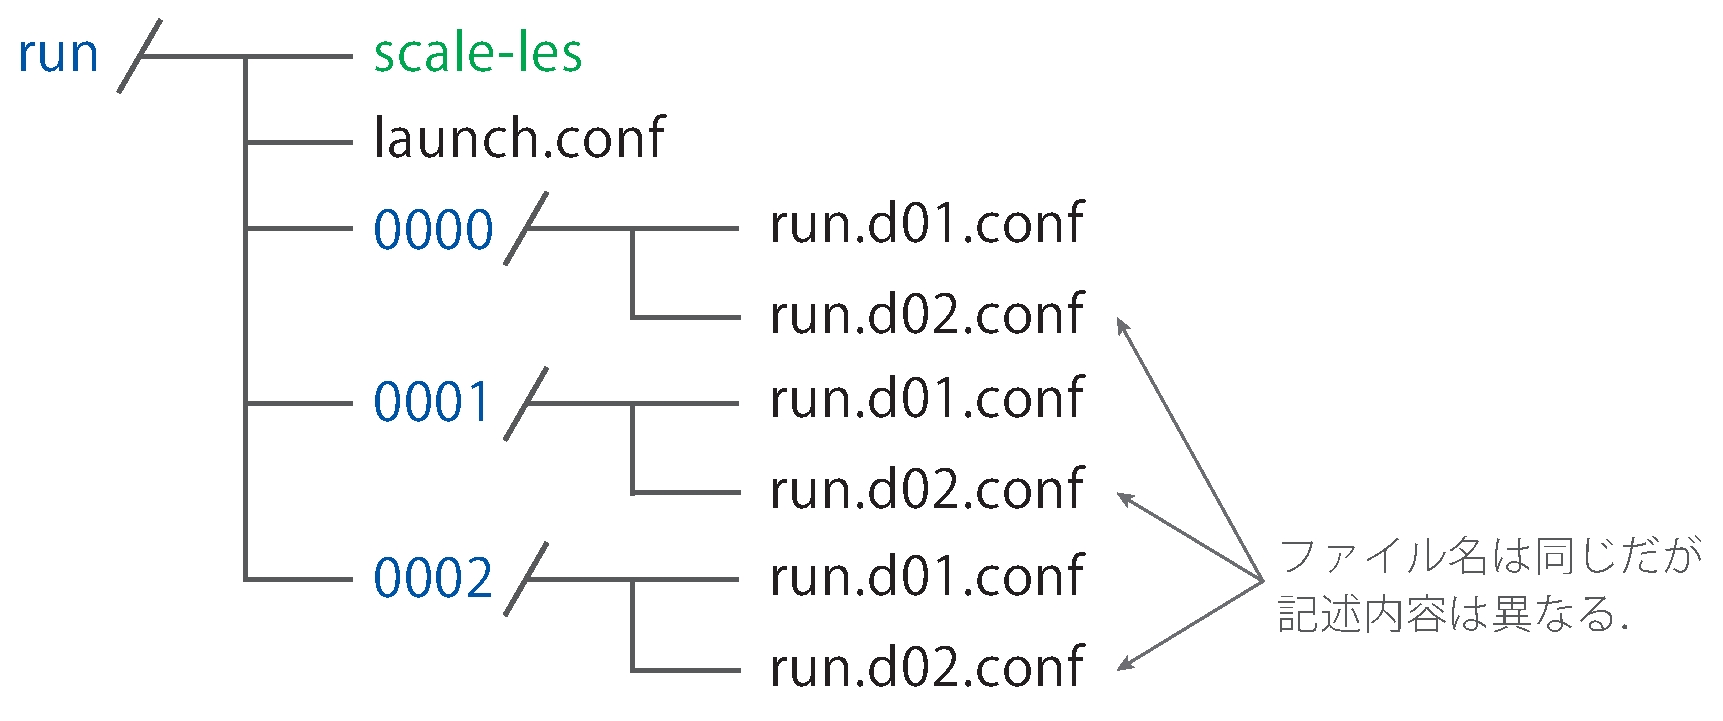
\includegraphics[width=0.6\hsize]{./figure/bulkjob_directory_structure.eps}\\
  \caption{バルクジョブ機能を使ってscale-lesを実行する場合のディレクトリ構造. ``0000''や``0001''はジョブ番号
           に対応する名前を持ったジョブディレクトリである。各ジョブディレクトリの中には、そこで実行する実験に関する
           configファイルが置かれている。データパラメタテーブルなどのファイルやディレクトリの記述は割愛しているが、
           それらも必要に応じて適切に配置する必要がある。}
  \label{fig_bulkjob}
\end{center}
\end{figure}


バルクジョブ実行するにあたって下記のものを事前に準備する必要がある。
\begin{itemize}
\item バルクジョブ用のディレクトリ構造
\item 実験に必要なすべてのconfigファイル
\item 実験に必要なすべての外部入力データ
\item 実行用のlaunch.confファイル
\end{itemize}

まず、図\ref{fig_bulkjob}に示すようなディレクトリ構造を準備する。``0000''や``0001''といったディレクトリは、
ジョブ番号に対応する名前を持ったジョブディレクトリである。ジョブディレクトリは必ず4桁の数字で、ジョブ番号はゼロから
数え上げられる。これらのディレクトリの中にはconfigファイルが収められている。
今回は2段オンライン・ネスティング実験を想定しているので、``run.d01.conf''と``run.d02.conf''の2つのファイルが準備
されている。各ジョブディレクトリにあるconfigファイルの名前は同じにする必要があるが、内容は異なっていても構わない。
ただし、\textcolor{red}{ドメイン毎に使用するMPIプロセス数は全てのジョブで共通していなければならない。}
configファイル内にバルクジョブ機能用に追加する設定項目はないが、\textcolor{red}{入出力ファイルのPATHを適切に
記述する}必要がある。以下にジョブ0000番のrun.d01.confの抜粋を示す。\\

\noindent {\small {\gt
\ovalbox{
\begin{tabularx}{140mm}{l}
\verb|&PARAM_IO| \\
\textcolor{blue}{\verb| IO_LOG_BASENAME = "0000/LOG_d01",|} \\
\verb|/| \\
 \\
\verb|&PARAM_RESTART| \\
\verb| RESTART_OUTPUT       = .true.,| \\
\textcolor{blue}{\verb| RESTART_OUT_BASENAME = "0000/restart_d01",|} \\
\textcolor{cyan}{\verb| RESTART_IN_BASENAME  = "../init/0000/init_d01_00013046400.000",|} \\
\verb|/| \\
 \\
\verb|&PARAM_TOPO| \\
\textcolor{cyan}{\verb| TOPO_IN_BASENAME = "../pp/0000/topo_d01",|} \\
\verb|/| \\
 \\
\verb|&PARAM_LANDUSE| \\
\textcolor{cyan}{\verb| LANDUSE_IN_BASENAME = "../pp/0000/landuse_d01",|} \\
\verb|/| \\
 \\
\verb|&PARAM_ATMOS_BOUNDARY| \\
\verb|     〜 中略 〜|\\
\textcolor{cyan}{\verb| ATMOS_BOUNDARY_IN_BASENAME    = "../init/0000/boundary_d01",|} \\
\verb|     〜 以下略 〜|\\
\verb|/| \\
 \\
\verb|&PARAM_HISTORY| \\
\textcolor{blue}{\verb| HISTORY_DEFAULT_BASENAME  = "0000/history_d01",|} \\
\verb|     〜 以下略 〜|\\
\verb|/| \\
\end{tabularx}
}}}\\

\noindent 上記のconfigファイルの設定例のうち、青色文字の部分は出力ファイルの指定、水色文字の部分は入力ファイルの指定である。
図\ref{fig_bulkjob}を見てわかるように、実行バイナリ(scale-les)があるのは``runディレクトリ''の下で、
ジョブディレクトリも実行バイナリと同じ階層にある。従って、ジョブ0000番において、実行バイナリからみてデータを出力するべき
ディレクトリは、``0000/''の下である。そこで出力ファイル名の指定として``0000/***''と記述している。

入力ファイルについても同様である。ここでは、runディレクトリと同じ階層にppディレクトリやinitディレクトリがあり、
その中にまたジョブディレクトリが作成してあって、それらの中に入力ファイルが保管されている状況を想定している。
従って、runディレクトリの下で実行される実行バイナリにとっては、``../pp/0000/***''といったPATHになる。

バルクジョブ機能は、オンライン・ネスティング実験で利用したMPIプロセスを分割・分配する機能を使って実装されている。
したがって、ジョブの起動のために``launch.conf''ファイルが必要になる。オンライン・ネスティング実験とバルクジョブ機能を
併用して実行する今回のような場合もlaunch.confファイルは1つだけで良い。\\

\noindent {\small {\gt
\ovalbox{
\begin{tabularx}{140mm}{l}
\verb|&PARAM_LAUNCHER| \\
\verb| NUM_BULKJOB = 3,| \\
\verb| NUM_DOMAIN  = 2,| \\
\verb| PRC_DOMAINS = 9,36,| \\
\verb| CONF_FILES  = run.d01.conf,run.d02.conf,| \\
\verb|/| \\
\end{tabularx}
}}}\\

\noindent 上記がオンライン・ネスティング実験とバルクジョブ機能を併用して実行する場合のlaunch.confファイルの中身である。
オンライン・ネスティング実験の場合のlaunch.confファイルに対して、\verb|NUM_BULKJOB|の設定項目を加えただけとなっている。
ここで実行するジョブ数は3つであるので、\verb|NUM_BULKJOB|に対して``3''と指定する。シングルドメイン実験として
バルクジョブ機能を利用する場合は、\verb|NUM_DOMAIN = 1|と指定して、\verb|CONF_FILES|に1つだけconfigファイルを指定すればよい。
実行時のコマンドは、 

\begin{verbatim}
 $ mpirun  -n  135  ./scale-les  launch.conf
\end{verbatim}

となる。ここでは1ジョブあたり、$9 + 36 = 45$プロセス使用し、全体で3つのジョブを実行するので、総計で135プロセスを
必要とする。

実行すると得られるLOGファイルに、MPIプロセスを分割した時の情報が示されている。LOGファイルを開いて最初の
「SCALEロゴ」のあとに下記のようなメッセージが出力される。\\

\noindent {\small {\gt
\ovalbox{
\begin{tabularx}{140mm}{l}
\verb| ++++++ Start MPI| \\
\verb| *** LOCAL_COMM_WORLD        :  4| \\
\verb| *** total process  [LOCAL]  :  12| \\
\verb| *** master rank    [LOCAL]  :  0| \\
\verb| *** my process ID  [LOCAL]  :  0| \\
\verb| *** GLOBAL_COMM_WORLD       :  3| \\
\verb| *** total process  [GLOBAL] :  48| \\
\verb| *** my process ID  [GLOBAL] :  36| \\
\verb| *** MASTER_COMM_WORLD       :  0| \\
\verb| *** total process  [MASTER] :  1488| \\
\verb| *** my process ID  [MASTER] :  36| \\
\end{tabularx}
}}}\\

これらのうち、\verb|[LOCAL]|と表記されている項目はドメイン内のプロセスグループ、\verb|[GLOBAL]|と表記されている項目は
ネスティング・グループ、\verb|[MASTER]|と表記されて項目はジョブ・グループに関する情報である。
したがって、このLOGメッセージから、当該ドメインは12-MPI並列で実行されており、オンライン・ネスティング実験は総計で
48プロセス使用して実行され、バルクジョブ全体では1488プロセスが使用されているため、同時に31個のジョブが走っていたことがわかる。
異常終了したときにも、この表記法に従ってメッセージが出力されるので、これを理解しているとバルクジョブ機能を使って多量に
走らせている場合にも、どのプロセスがエラーを発生したのか即座に判断できる。ちなみに現在のバルクジョブ機能では、
1つのジョブがエラーを発生し、異常終了状態に入ると全てのジョブが異常終了する。
以上でバルクジョブ機能の説明を終える。


%%%%%%%%%%%%%%%%%%%%%%%%%%%%%%%%%%%%%%%%%%%%%%%%%%%%%%%%%%%%%%%%%%%%%%%%%%%%%%%%%%%%%%
